% #############################################################################
% This is Chapter 6
% !TEX root = ../main.tex
% #############################################################################
% Change the Name of the Chapter i the following line
\fancychapter{System Evaluation}
\cleardoublepage
% The following line allows to ref this chapter
\label{chap:evaluation}

This chapter concerns the system and board evaluation. The system and board were evaluated regarding its performance and the fullfilled requirements outlined in the previous project report and the problem definition chapter \ref{chap:problem}.
% -----------------------------------------------------
% -----------------------------------------------------
\section{Performance Tests}\label{chap:evaluation:performance}

The test objectives, configuration, results and conclusions are detailed for every tested component.
The communication channel, smartfusion2 board's security services and implemented services were tested.
Two performance metrics were calculated, the test processing time, and the tested component's throughput.

% -----------------------------------------------------
\subsection{Testing configuration}\label{chap:evaluation:performance:config}

The tests were all performed on a Windows 10 computer, connected to the smartfusion2 device through a \ac{UART} serial port. The implemented PKCS\#11 program interface was used to run the tests.
Two programs were running on the computer while performing the tests, the PKCS\#11 interface program and the SoftConsole IDE to run the code on the smartfusion board.
For all tests, the serial port UART connection was configured with a 115200 bit/s baud rate.%, 8 data bits, no parity bits and one stop bit.
Since the board does not provide a clock and \ac{API} to measure elapsed time, the time has to be measured in the interface software side.
The elapsed time was measured using the function \texttt{gettimeofday()} available in the C library \texttt{sys/time.h}.
Time measurement starts right before sending a message to the device which triggers the operation, and stops when the client receives a message from the device, after the operation is finished.
In order to thoroughly study the performance and scalability of each component, the transmitted data size was varied, only for components where it is logical and can potentially have a performance impact. The data size was tested, when possible, up to 36 KBytes. The size is limited by the device's \ac{RAM} of 64 KB.
Tests were performed in two different configurations.
Obvious outlier values were excluded from the experimental calculations. The adopted rule was that values which are significantly above or below the average, and are never repeated were eliminated from the sample set.
For the first test configuration, the measured operation is performed once in the device each transmission. This transmission is repeated multiple times for every set of values, until an acceptable variance is achieved. For most components the variance is well bellow 1\%. % The more volatile test results have a variance below 4\%.
For most components the first configuration produced unstable results with a high variance, due to the communications overhead on every test run.
Thus, a second test configuration was applied on components where the time to transmit messages needs to be minimized to more accurately assess its performance. For each transmission, the operation was performed 100 consecutive times in the board. The resulting time was divided by 100 to obtain the average processing time of the operation.
With the second configuration, the tests are visibly more stable.
A test example of the difference between both configurations results was on testing the \ac{AES} security service. The first scenario's communication overhead was on average 15\% compared to the second configuration results, with a peak 61\% overhead for small data sizes. Additionally when plotting the results, the second results scale almost perfectly linear, and the first results' are significantly more unstable.

% -----------------------------------------------------
\subsection{Communications}\label{chap:evaluation:performance:comms}

In order to assess the communication channel performance, and its impact on the system, the average time to transmit data was measured. For each test, the interface sent some data of a specific size to the device, and it returned an acknowledge message on reception. The test, in accordance with the first scenario, was repeated at least 30 times for each data size. The highest variance did not go above 0.2\%.
The average transmission times for each value are displayed in figure \ref{fig:comms:time}.
The values range from 0.048 seconds for 0.5 KB, to 3.2 s for 36 KB.
From the graph we can conclude the performance has linear scalability.

\begin{figure}[h!]
	\centering
	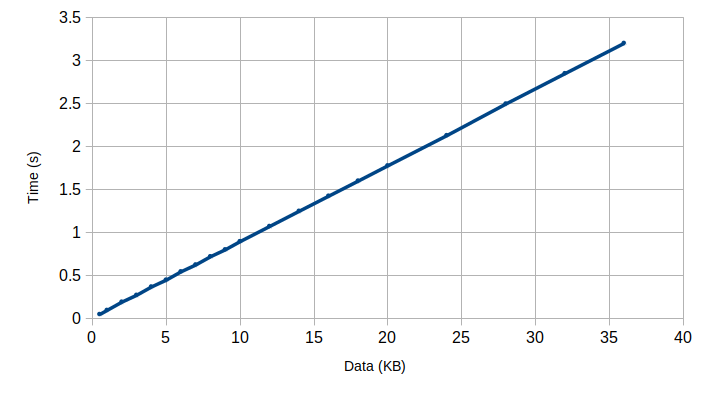
\includegraphics[width=0.8\textwidth]{./Images/comms-time.png}
	\caption{Average Data Transmission Times}
	\label{fig:comms:time}
\end{figure}

For the subsequent graphic, the throughput was calculated from the transmission tests, for every repetition.
Figure~\ref{fig:comms:tput} plots the experimental throughput and theoretical throughput. The theoretical throughput was calculated from the baud rate \(115200/8 = 14.06 KBytes/s\).
We observe the experimental throughput starts at around 10 KB/s for smaller data sizes and stabilizes around 11 KB/s as data size increases.
We can conclude the practical throughput is close to the theoretical, and as expected stabilizes as the data size increases.

\begin{figure}[h!]
	\centering
	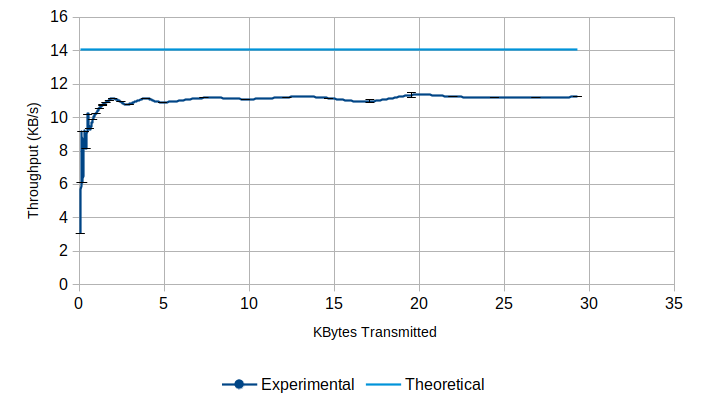
\includegraphics[width=0.8\textwidth]{./Images/comms-tput.png}
	\caption{Serial Port Communications Throughput}
	\label{fig:comms:tput}
\end{figure}

% -----------------------------------------------------
% -----------------------------------------------------
\subsection{Smartfusion2 Security Services}\label{chap:evaluation:board}

\begin{equation}
	\label{eq:linear-eq}
	Ttotal = Tcall + Tdata * KBytes
\end{equation}

\begin{table}[h!]
\centering
\def\arraystretch{1.5}
\begin{tabular}{|c|c|c|c|c|c|c|c|}
\hline
Time (ms) & AES    & SHA    & HMAC   & TRNG   & KeyTree & ECC Add. & ECC Mult.	\\ \hline
Constant  & 0.489  & 0.498  & 0.783  & 0.368  & 1.655   & 7.204    & 545.381	\\ \hline
Data (KB) & 11.124 & 0.807  & 7.815  & 0.007  & -       & -	   & -		\\ \hline
MAE       & 0.12\% & 0.84\% & 0.13\% & 2.29\% & -       & -	   & -		\\ \hline
\end{tabular}
\caption{SmartFusion2 services time performance according to a linear model}
\label{tab:core-model}
\end{table}


% TODO
\begin{figure}[h!]
	\centering
	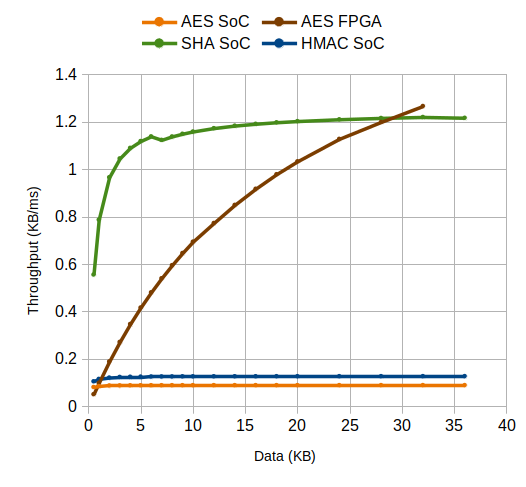
\includegraphics[width=0.9\textwidth]{./Images/core-tput.png}
	\caption{TODO}
	\label{fig:performance:core-tput}
\end{figure}

% -----------------------------------------------------
% -----------------------------------------------------
\subsection{Implemented Services}\label{chap:evaluation:services}

The same library used to measure the time in the communication tests was used.
The time was measured at the client application before sending the message which will trigger the service at the HSM, and after it has received the result.

In order to get a real time measurement, each operation was performed 1000 times on the HSM, with the communications only done once.
From the resulting time, the predicted time spent on communications was subtracted using the data from the previous test. The result was then divided by 1000.

The data encryption and decryption operations were ran with different data sizes, in order to asses the data size impact on performance.
The ECDH key generation always uses a private and public key of the same size, so no message size variation is possible.

\begin{table}[h!]
\centering
\def\arraystretch{1.5}
\begin{tabular}{|c|c|c|c|c|c|c|}
\hline
	Time (ms) & Encrypt Data  & Decrypt Data  & Import Keys & ECDSA & ECDH   \\ \hline
	constant  & 2.1    & 0.847  & 368.994  & 629.932 & 964.535 \\ \hline
	data      & 14.678 & 14.681 & 18.518 & 0.937 & - \\ \hline
	MAE	  & 0.10\% & 0.12\%  & 2.86\% & 0.18\% & - \\ \hline
\end{tabular}
\caption{Implemented services time values according to a linear model}
\label{tab:services-model}
\end{table}

% \begin{table}[]
% \centering
% \def\arraystretch{1.5}
% \begin{tabular}{|c|c|c|c|c|c|c|}
% \hline
% Time/Service   & Encrypt + MAC	  & Decrypt + MAC  & Import Keys & ECDSA   \\ \hline
%         constant (ms) & 29.413 & 29.413 & 0.002 & 0.138 \\ \hline
%         data (ms) & 6.704 & 6.704 & 1.942 & 1.542 \\ \hline
%         MAE \%	   & 1.032 & 1.006 & 0.127 & 1.760 \\ \hline
% \end{tabular}
% \caption{Implemented services throughput model values}
% \label{tab:services-model}
% \end{table}


% TODO
\begin{figure}[h!]
	\centering
	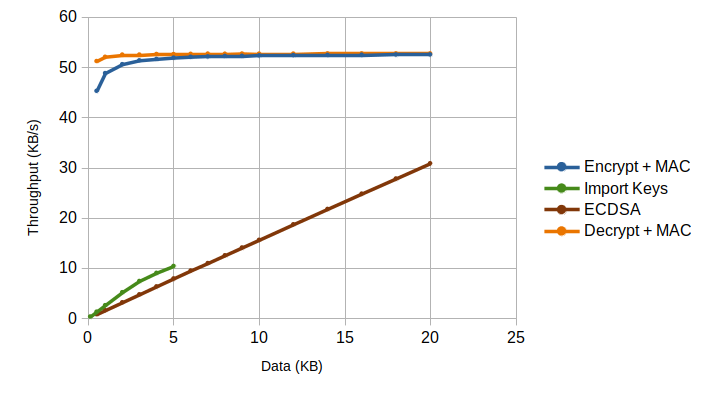
\includegraphics[width=0.9\textwidth]{./Images/services-tput.png}
	\caption{TODO}
	\label{fig:performance:services-tput}
\end{figure}

% TODO
The results in table~ for the encryption and decryption operations are very similar due to both using the same board services, AES encryption and HMAC, but in a different order. It is also important to note AES encryption and decryption in CTR mode is essentially the same operation due the mode's characteristics.
Relating to the variation in data size, the values vary between approximately 0.1284 and 0.1825 seconds, which is a very insignificant difference. Thus we can conclude, the data size has a negligible impact on the operations performance.

% TODO
Regarding the key generation operation results in table~, two values were obtained through different methods. Due to the operation using SRAM-PUF services to enroll new keys in the eNVM memory, with limited write cycles and key slots, this operation cannot be repeated enough times to get a relevant enough sample size.
So a trade off was achieved. The operation was performed 1000 times without the key enrollment operation, meaning only the ecdh key generation algorithm and key derivation function (SHA-256).
Since the enrollment phase is presumed to be expensive, due to writing in eNVM memory, the test was also performed 10 times with key enrollment, to get an idea of its potential performance cost.

A higher time of 0.577 seconds without enrollment and 1.764s with, compared to the previous operations is expected due to the higher cost of operations with asymmetric keys.
However, comparing both values we can conclude saving the key in memory, has most likely the higher performance impact on the operation.
This result is congruent with the one obtained by \cite{parrinha2017flexible} of 0.57s per ECC scalar multiplication.
Thus we can conclude, the scalar multiplication is the second most expensive operation, after the key enrollment, since the key derivation function has a negligible impact on the processing time (0.577s with the function vs 0.57s without).

% -----------------------------------------------------
% -----------------------------------------------------
\section{Requirements}\label{chap:evaluation:requirements}

A M2S090TS smartfusion2 evaluation kit is priced at 384€ \cite{smartfusionPrice}.

% ------------- Requirements ------------------
% Devices should be distributable to individuals or entities with one or more individuals;
% The system must allow communications between individuals representing themselves or an entity;
% The system must be responsible for securing all communications against any sort of attacks;
% The device should be independent from user's personal computers;
% Users should be able to create secure communications with available and new entities;
% m New secure connections should be created, if existing communications are suspected to be compromised;
% It should provide an easy-to-use interface by everyone, including non-technical people;
% It should have a relatively low cost, to allow distribution of several devices among multiple people;
% Only authorized individuals should be able to use the device.
% ---------------------------------------------

% secure comms - aes and hmac services are not dpa resistant, so keys should be regularly replaced to avoid enough data which enables an attacker to break encryption. On the other hand this is only possible if the attacker has physical access to the device or potentially with some type of malware on the user's computer.
% key generation - needs assymetric keys to generate new keys with public keys and salt traded beforehand - can be not user friendly

% -----------------------------------------------------
% -----------------------------------------------------
\section{Summary}\label{chap:evaluation:summary}
